% Provenance (never printed): see sources/outline_sources.md (Year 1: morphology,
% gravity, heat flow and seismicity of a subduction zone; accretionary and erosive
% margins; slab geometry; volcanic arcs). Kuril map, section and numbers from
% figdata/bachelor-1/slab_seismicity.py; exercise and problem values in the Book 3
% scratch calculator calc/ch14.py.
\chapter{Active Margins}\label{ch:b1:active-margins}

On 11 March 2011, at 14:46 local time, the plate boundary off north-east Japan
broke over some \qty{400}{km} along the trench and \qty{150}{km} down its \omterm{def:b1:geological-maps:attitude}{dip}.
The fault slipped by as much as 50 to \qty{60}{m}, most of it \omterm{def:b1:geological-maps:attitude}{up-dip} of the
hypocentre, towards the Japan Trench; on land, the coast moved horizontally and
subsided. The plate that sinks there, the Pacific plate, goes down beneath
Japan along a plane that earthquakes outline down to hundreds of kilometres;
and where that plane lies about a hundred kilometres deep, a line of volcanoes
runs parallel to the coast. This chapter reads such a margin from its shape,
its gravity, its \omterm{def:b1:heat-budget:heat-flow}{heat flow} and, above all, its earthquakes.
% ledger: usgs:tohoku, wada:decoupling

\begin{recall}
Oceanic \omterm{def:b1:layered-earth:lithosphere}{lithosphere} sinks back into the \omterm{def:b1:layered-earth:layers}{mantle} at subduction zones, marked by
trenches and by inclined zones of earthquakes, and old \omterm{def:b1:layered-earth:lithosphere}{lithosphere} sinks under
its own weight (Book 2, grade 11); water from the sinking plate lowers the
melting temperature of the \omterm{def:b1:layered-earth:layers}{mantle} above it (Book 2, grade 12). Heat diffuses
over a distance $L$ in a time of order $L^2/\kappa$ (\cref{ch:b1:heat-budget});
an infinite slab of density $\rho$ and thickness $h$ attracts with $2\pi G\rho h$
(\cref{ch:b1:isostasy-gravity}); plates move about \omterm{def:b1:plate-kinematics:euler-pole}{Euler poles}
(\cref{ch:b1:plate-kinematics}); the \omterm{def:b1:heat-budget:heat-flow}{heat flow} of the ocean floor falls as the
inverse square root of its age (\cref{ch:b1:rifts-ridges-margins}).
\end{recall}

\section{The anatomy of an active margin}\label{sec:b1:active-margins:anatomy}

\begin{definition}[Active margin, oceanic trench, forearc, back-arc basin]\label{def:b1:active-margins:active-margin}
An \emph{active margin}\index{active margin} is a convergent plate boundary at
which oceanic \omterm{def:b1:layered-earth:lithosphere}{lithosphere} sinks beneath another plate, either beneath a
continent or beneath another oceanic plate. An \emph{oceanic
trench}\index{oceanic trench} is the long, narrow, V-shaped depression of the
sea floor along which the sinking plate bends down beneath the other. The
\emph{forearc}\index{forearc} is the part of the overriding plate between the
trench and the line of volcanoes. A \emph{back-arc basin}\index{back-arc basin}
is a basin behind the volcanoes, on the side away from the trench, where the
overriding plate is stretched and new \omterm{def:b1:rifts-ridges-margins:oceanic-crust}{oceanic crust} may form.
\end{definition}

Trenches are the deepest places of the oceans, and the deepest of all is the
Challenger Deep of the Mariana Trench. Across the Kuril Trench the floor drops
from about \qty{5200}{m} on the abyssal plain to \qty{8700}{m} at the axis,
some \qty{3.5}{km} lower, and the trench is only tens of kilometres wide
(figure in \cref{sec:b1:active-margins:gravity-heat}). The convergent margins
of the Earth measure about \qty{55000}{km} in all; in a digital model of the
plate boundaries the subduction boundaries add up to about \qty{51000}{km},
against about \qty{67000}{km} of spreading ridges.
% ledger: data:b3-grav-kuril (trench_gravity.py values), stern:subduction, data:pb2002 (ridge_budget.py)

Seaward of the trench the plate rises slightly before it \omterm{def:b1:field-lab-methods-1:trend-plunge}{plunges}, in a broad,
low outer rise. There the plate is bent, and its upper part is stretched:
earthquakes of normal faulting strike the outer rises. The width of the outer
rise matches the bending of an elastic plate; this flexure of the \omterm{def:b1:layered-earth:lithosphere}{lithosphere}
is studied in Book 5. The trench itself is the place where the weight of the
dense sinking plate pulls its leading edge down.

\begin{definition}[Subducting slab]\label{def:b1:active-margins:slab}
The \emph{subducting slab}\index{subducting slab} is the part of the sinking
plate that has already gone down into the \omterm{def:b1:layered-earth:layers}{mantle}: a sheet of oceanic
\omterm{def:b1:layered-earth:lithosphere}{lithosphere}, with its \omterm{def:b1:layered-earth:layers}{crust} on top, inclined beneath the overriding plate from
the trench to depths of several hundred kilometres.
\end{definition}

The overriding plate is cut into strips parallel to the trench
(figure below): the \omterm{def:b1:active-margins:active-margin}{forearc}, often with a pile of
scraped-off sediments at its front and a sedimentary basin behind; the
\omterm{def:b1:active-margins:volcanic-arc}{volcanic arc}; and, behind some arcs, a \omterm{def:b1:active-margins:active-margin}{back-arc basin} and an older, extinct
arc beyond it. Between the slab and the overriding plate lies a wedge of
\omterm{def:b1:layered-earth:layers}{mantle}, dragged down along the top of the slab.

\begin{omfigure}
\begin{tikzpicture}[x=0.01667cm, y=0.01667cm, font=\scriptsize,
  lbl/.style={fill=white, fill opacity=0.8, text opacity=1, inner sep=1pt}]
\begin{scope}
\clip (-150,-330) rectangle (650,55);
% mantle and sea water
\fill[orange!12] (-150,-330) rectangle (650,15);
\fill[omSea!45] (-150,15) rectangle (650,0);
% incoming plate and slab: top dips 25 deg to 50 km, then 45 deg; 100 km thick
\fill[omLithBasalt!55] (-150,4) -- (-80,4) .. controls (-60,7) and (-40,7) .. (-25,4) -- (0,0)
  -- (107.2,-50) -- (420,-363) -- (349,-434) -- (48.9,-133.1) -- (-22.1,-100) -- (-150,-100) -- cycle;
\draw[omSea!50!black, line width=1.6pt] (-150,4) -- (-80,4) .. controls (-60,7) and (-40,7) .. (-25,4) -- (0,0) -- (107.2,-50) -- (420,-363);
% overriding plate
\fill[brown!28] (0,0) -- (12,3) -- (45,8) -- (60,10) -- (140,10) -- (150,12) -- (184,12) -- (230,9)
  -- (300,7) -- (395,6) -- (410,3) -- (420,2) -- (430,3) -- (445,6) -- (540,7) -- (560,14) -- (590,14)
  -- (610,10) -- (650,10) -- (650,-60) -- (520,-55) -- (445,-25) -- (420,-15) -- (395,-25) -- (320,-55)
  -- (250,-60) -- (117.2,-60) -- (107.2,-50) -- cycle;
% accretionary prism and forearc basin
\fill[yellow!55] (0,0) -- (12,3) -- (45,8) -- (60,10) -- (60,-28) -- cycle;
\draw[black!45, line width=0.3pt] (14,-3) -- (24,5) (28,-7) -- (38,6) (42,-14) -- (52,8);
\fill[yellow!30] (68,10) -- (132,10) -- (122,4) -- (78,4) -- cycle;
% arc volcano
\fill[black!60] (150,12) -- (167,26) -- (184,12) -- cycle;
% an isotherm: a cold tongue down the slab
\draw[omDef, dashed, line width=0.6pt] (-150,-82) -- (-30,-82) -- (40,-118) -- (300,-318)
  -- (232,-200) -- (150,-112) .. controls (130,-80) and (180,-72) .. (260,-72) -- (650,-72);
% mantle wedge flow
\draw[->, black!60, line width=0.5pt] (600,-130) .. controls (450,-135) and (300,-125) .. (215,-150)
  .. controls (205,-160) and (240,-185) .. (300,-235);
% water and melt
\foreach \x/\z in {150/-93, 172/-115, 194/-137}
  \draw[->, blue!70!black, line width=0.5pt] (\x,\z) -- (\x-6,\z+28);
\draw[red!75!black, line width=0.8pt, decorate, decoration={snake, amplitude=1.2, segment length=6}] (167,-100) -- (167,12);
% earthquakes
\foreach \x/\z in {20/-12, 45/-22, 70/-34, 95/-45, 60/-40, 85/-58, 120/-70, 135/-85, 150/-104,
  165/-112, 185/-140, 205/-150, 225/-175, 248/-195, 270/-216, 290/-242, 312/-262, 330/-282, 350/-300, 365/-318}
  \fill[black] (\x,\z) circle[radius=0.9pt];
% the 100-km level beneath the arc
\draw[black!70, densely dotted] (90,-100) -- (260,-100);
\draw[black!70, densely dotted] (167,12) -- (167,-110);
\end{scope}
\draw[black!70] (-150,-330) rectangle (650,55);
\node[lbl, anchor=south] at (-85,15) {outer rise};
\node[lbl, anchor=south] at (0,15) {trench};
\node[lbl, anchor=west] (pr) at (75,-28) {accretionary prism};
\draw[black!70] (pr.west) -- (38,-6);
\node[lbl, anchor=south] at (88,15) {forearc};
\node[lbl, anchor=south] at (185,27) {volcanic arc};
\node[lbl, anchor=south] at (420,15) {back-arc basin};
\node[lbl, anchor=south] at (575,15) {remnant arc};
\node[lbl, anchor=west] at (-140,-50) {oceanic lithosphere};
\node[lbl, anchor=east] (sl) at (120,-262) {subducting slab};
\draw[black!70] (sl.east) -- (205,-262);
\node[lbl, anchor=west] (wb) at (420,-265) {Wadati--Benioff zone};
\draw[black!70] (wb.west) -- (318,-266);
\node[lbl] at (430,-170) {mantle wedge};
\node[lbl] at (575,-30) {overriding plate};
\node[lbl, anchor=west, text=blue!70!black] at (212,-98) {water};
\node[lbl, anchor=east] at (88,-100) {\qty{100}{km} deep};
\node[lbl, anchor=west, text=omDef] at (450,-95) {an isotherm};
\node[lbl, anchor=west] at (-140,-300) {mantle};
\draw[line width=1pt] (500,-310) -- (600,-310) node[midway, above] {\qty{100}{km}};
\end{tikzpicture}
\par\smallskip{\small A subduction zone in section (schematic: \omterm{def:b1:layered-earth:lithosphere}{lithosphere} and
slab drawn to the scale bar, relief above the sea floor greatly exaggerated).
The slab \omterm{def:b1:geological-maps:attitude}{dips} gently beneath the \omterm{def:b1:active-margins:active-margin}{forearc} and more steeply below; the \omterm{def:b1:active-margins:volcanic-arc}{volcanic
arc} stands above the place where the top of the slab is about \qty{100}{km}
deep. The cold slab drags its isotherms down into the \omterm{def:b1:layered-earth:layers}{mantle} (dashed: one
isotherm), and the \omterm{def:b1:layered-earth:layers}{mantle} of the wedge is dragged down along it. Dots:
earthquakes, on the plate boundary near the trench and inside the slab below.
Water released by the slab rises into the wedge; melt rises to the arc.}
\label{fig:b1:active-margins:section}
\end{omfigure}

Summed over the same digital model, about \qty{2.7}{km^2} of ocean floor go
down the subduction boundaries each year, close to the \qty{3.0}{km^2} made at
the ridges (\cref{ch:b1:rifts-ridges-margins}): within the accuracy of such a
model, which leaves out the slow deformation of wide plate-boundary zones, the
ocean floor is destroyed as fast as it is made, and the surface of the Earth
keeps its size.
% ledger: data:pb2002 (ridge_budget.py: consumed 2.74, made 3.01 km2/yr)

\section{Gravity and heat flow}\label{sec:b1:active-margins:gravity-heat}

Felix Vening Meinesz found the long, narrow belts of negative gravity anomalies
along the trenches (\cref{ch:b1:isostasy-gravity}). Satellites now map them
everywhere at sea. Across the Kuril Trench (figure below) the \omterm{def:b1:isostasy-gravity:anomalies}{free-air anomaly}
rises to about \qty{40}{\milli\gal} over the outer rise, falls to
\qty{-260}{\milli\gal} over the trench, and is strongly positive again over the
\omterm{def:b1:active-margins:active-margin}{forearc} and the islands of the arc.
% ledger: egs:vening-meinesz, data:b3-grav-kuril (trench_gravity.py values: rise 38 mGal at -155 km, low -260 at 0, high 218 at 160 km)

The size of the trench anomaly tells how the trench is held. Suppose the trench,
\qty{3.5}{km} deeper than the floor around it, were not compensated at all:
where the trench is, \qty{3.5}{km} of rock of density about
\qty{2700}{kg.m^{-3}} is replaced by sea water. By the Bouguer slab
(\cref{prop:b1:isostasy-gravity:slab}) gravity there would be lower by
\[
  2\pi G\,\Delta\rho\,h = 2\pi \times \num{6.674e-11} \times 1700 \times 3500
  \approx \qty{2.5e-3}{m.s^{-2}} = \qty{250}{\milli\gal} .
\]
That is the size of the observed low. A trench is therefore not in isostatic
equilibrium: it is a depression held down, by the strength of the bent plate
and by the pull of the slab, against the buoyancy of the \omterm{def:b1:layered-earth:layers}{mantle} below. (A
trench only tens of kilometres wide attracts less than an infinite slab, so
the water in it alone gives somewhat less than this; the rest of the deficit
lies deeper, where the whole bent plate, its light \omterm{def:b1:layered-earth:layers}{crust} included, is pushed
down into the \omterm{def:b1:layered-earth:layers}{mantle}: exercise~\ref{exo:b1:active-margins:1}.)

\begin{omfigure}
\begin{tikzpicture}
\begin{axis}[omrecord, name=grav, width=0.86\linewidth, height=4.6cm, xmin=-250, xmax=450,
  ymin=-300, ymax=260, ylabel={free air (\unit{\milli\gal})}, ylabel style={at={(-0.075,0.5)}}, xticklabels={},
  ytick={-200,-100,0,100,200}, clip=false]
% computed in figdata/bachelor-1/trench_gravity.py; ledger: data:b3-grav-kuril
\addplot[black!30, forget plot] coordinates {(-250,0) (450,0)};
\addplot[omDef, line width=1pt] table[x=x, y=faa] {figdata/out/bachelor-1-trench_gravity-profile.dat};
\draw[black!50, densely dotted] (axis cs:0,-300) -- (axis cs:0,260) (axis cs:164,-300) -- (axis cs:164,260);
\node[font=\scriptsize, anchor=south] at (axis cs:-155,45) {outer rise, $+38$};
\node[font=\scriptsize, anchor=west] at (axis cs:12,-262) {trench, $-260$};
\node[font=\scriptsize, anchor=south west] at (axis cs:200,140) {forearc and arc};
\end{axis}
\begin{axis}[omrecord, at={(grav.south)}, anchor=north, yshift=-0.45cm, width=0.86\linewidth, height=4.6cm,
  xmin=-250, xmax=450, ymin=20, ymax=100, ylabel={heat (\unit{mW.m^{-2}})}, ylabel style={at={(-0.075,0.5)}},
  xlabel={distance from the trench, toward the overriding plate (\unit{km})}, clip=false]
% schematic; levels from the ledger: parsons:plate-model (11.3/sqrt(122) x 41.84 = 42.8 mW/m2 for the
% 122-Myr Kuril plate), hyndman:backarc (70-85); the forearc low is drawn without a value (wada:decoupling)
\addplot[fill=omDef!15, draw=none, forget plot] coordinates {(190,70) (450,70) (450,85) (190,85)} -- cycle;
\addplot[omProp!80!black, line width=1pt, smooth, tension=0.5] coordinates {(-250,43) (-60,43) (-10,41) (30,36) (120,36)
  (150,48) (180,76) (230,78) (450,78)};
\draw[black!50, densely dotted] (axis cs:0,20) -- (axis cs:0,100) (axis cs:164,20) -- (axis cs:164,100);
\node[font=\scriptsize, anchor=south] at (axis cs:-130,44) {old ocean floor, about 43};
\node[font=\scriptsize, anchor=north] at (axis cs:75,34) {forearc: lower};
\node[font=\scriptsize, anchor=south] at (axis cs:320,85) {arc and back-arc, 70 to 85};
\node[font=\scriptsize, anchor=north west] at (axis cs:3,99) {trench};
\node[font=\scriptsize, anchor=north west] at (axis cs:167,99) {arc};
\end{axis}
\end{tikzpicture}
\par\smallskip{\small Gravity and \omterm{def:b1:heat-budget:heat-flow}{heat flow} across a subduction zone. Top: the
free-air \omterm{def:b1:isostasy-gravity:anomalies}{gravity anomaly} measured by satellite across the Kuril Trench, along
the section of the figure in \cref{sec:b1:active-margins:seismicity}:
\qty{38}{\milli\gal} over the outer rise, \qty{-260}{\milli\gal} over the
trench, strongly positive over the \omterm{def:b1:active-margins:active-margin}{forearc} and the islands. Bottom: \omterm{def:b1:heat-budget:heat-flow}{heat flow},
a schematic profile: about \qty{43}{mW.m^{-2}} on the old ocean floor, lower
over the \omterm{def:b1:active-margins:active-margin}{forearc}, 70 to \qty{85}{mW.m^{-2}} on average over the arc and the
back-arc. Dotted: the trench and the volcanic front. Data: Scripps
Institution of Oceanography marine gravity model (Sandwell and others, 2014).}
\label{fig:b1:active-margins:profiles}
\end{omfigure}

The \omterm{def:b1:heat-budget:heat-flow}{heat flow} tells the same story from the other side. The old ocean floor
that comes to a trench loses little heat: about \qty{43}{mW.m^{-2}} by the law
of \cref{ch:b1:rifts-ridges-margins} for the Kuril plate, \qty{122}{Myr} old.
Over the \omterm{def:b1:active-margins:active-margin}{forearc} the flow is lower still: the cold slab beneath it takes up
heat from above, and the \omterm{def:b1:layered-earth:layers}{mantle} under the \omterm{def:b1:active-margins:active-margin}{forearc} is cold and stagnant. Over the arc
and the back-arc it is high, 70 to \qty{85}{mW.m^{-2}} on average, twice the
flow of the old interiors of continents (about \qty{40}{mW.m^{-2}}). An active
\omterm{def:b1:active-margins:volcanic-arc}{volcanic arc} needs a \omterm{def:b1:layered-earth:layers}{mantle} wedge at about \qty{1200}{\celsius} some
\qty{100}{km} down; behind it the whole back-arc is hot, with a \omterm{def:b1:layered-earth:lithosphere}{lithosphere}
only 50 to \qty{60}{km} thick and its \omterm{def:b1:layered-earth:discontinuity}{Moho} at 800 to \qty{900}{\celsius}.
% ledger: parsons:plate-model (11.3/sqrt(122) x 41.84 = 42.8), wada:decoupling, hyndman:backarc

Why does the slab stay cold? It sinks faster than it can warm up. The Kuril
slab of \cref{sec:b1:active-margins:seismicity} enters at about
\qty{82}{mm} a year and \omterm{def:b1:geological-maps:attitude}{dips} at \ang{45}: it reaches \qty{600}{km} after a path
of $600/\sin\ang{45} \approx \qty{850}{km}$, in about ten million years. By the
conductive time scale (\cref{prop:b1:heat-budget:timescale}), heat from the
\omterm{def:b1:layered-earth:layers}{mantle} crosses the \qty{50}{km} to the middle of a slab \qty{100}{km} thick in
\[
  \tau = \frac{L^2}{\kappa} = \frac{(\qty{5e4}{m})^2}{\qty{e-6}{m^2.s^{-1}}}
  = \qty{2.5e15}{s} \approx \qty{80}{Myr},
\]
about eight times longer. The core of the slab arrives at \qty{600}{km} almost as
cold as it was at the trench, and the isotherms are dragged down with it, as
the section of a subduction zone above shows.
% values (slab_seismicity.py): vel_normal 81.66 mm/yr, dip 44.9; calc/ch14.py

\section{Earthquakes and the shape of the slab}\label{sec:b1:active-margins:seismicity}

\begin{definition}[Wadati--Benioff zone]\label{def:b1:active-margins:wadati-benioff}
A \emph{Wadati--Benioff zone}\index{Wadati--Benioff zone} is the inclined zone
of earthquakes that starts near a trench and deepens beneath the overriding
plate, down to as much as about \qty{700}{km}: it outlines the \omterm{def:b1:active-margins:slab}{subducting slab}.
\end{definition}
% ledger: usgs:deepest

Its earthquakes are of two kinds. Down to some tens of kilometres they happen on
the plate boundary itself, the gently dipping fault along which the two plates
slide past each other; the largest earthquakes on Earth, such as that of 2011
off Japan, break this fault. Deeper, they happen inside the slab, which alone is
still cold enough to store stress. At the greatest depths even the slab should
flow rather than break, and how deep earthquakes start is still debated. The
deepest earthquake of the catalogue, of magnitude 4.2, struck beneath the
Vanuatu region in 2004 at \qty{735.8}{km}. In every subduction zone examined,
the zone is double at intermediate depths: two layers of earthquakes, further
apart in older plates.
% ledger: usgs:deepest, brudzinski:double, usgs:tohoku

The Kuril Islands, between Hokkaido and Kamchatka, sit above a slab that
earthquakes outline from the trench down to more than \qty{600}{km}. There the Pacific plate, about 120 million years old where it
reaches the trench, sinks beneath the Okhotsk plate
(map below). The earthquakes of magnitude 5 or more since
1976 draw the slab in plan: shallow ones along the trench, intermediate ones
beneath the islands, deep ones under the Sea of Okhotsk. On 24 May 2013 an
earthquake of magnitude 8.3 struck \qty{598}{km} beneath the Sea of Okhotsk,
in the same slab farther north; it was felt as far as Moscow, some
\qty{6400}{km} away.
% values (slab_seismicity.py): age_in 121.8 Myr (median of the cells 100-400 km seaward)
% ledger: data:b3-usgs-kuril, data:b2-seafloor-age, data:pb2002, usgs:okhotsk-2013

\begin{omfigure}
\begin{tikzpicture}
\begin{axis}[x=0.40cm, y=0.598cm, xmin=138, xmax=165, ymin=40, ymax=56,
  axis background/.style={fill=omSea!35}, axis on top,
  xtick={140,145,...,165}, ytick={40,45,...,55},
  xticklabel={$\pgfmathprintnumber{\tick}^\circ$E}, yticklabel={$\pgfmathprintnumber{\tick}^\circ$N},
  tick label style={font=\scriptsize}, grid=major, grid style={gray!25, line width=0.25pt},
  legend style={font=\scriptsize, at={(0.98,0.02)}, anchor=south east, cells={anchor=west}},
  clip=true]
% computed in figdata/bachelor-1/slab_seismicity.py; ledger: data:b3-usgs-kuril, data:gvp, data:pb2002
\addplot[fill=omLithAlluv, draw=black!45, line width=0.2pt, unbounded coords=jump, forget plot] table {figdata/out/bachelor-1-slab_seismicity-map-land.dat};
\addplot[only marks, mark=*, mark size=0.45pt, black!35] table {figdata/out/bachelor-1-slab_seismicity-map-qshallow.dat};
\addlegendentry{shallower than \qty{70}{km}}
\addplot[only marks, mark=*, mark size=0.8pt, orange!85!black] table {figdata/out/bachelor-1-slab_seismicity-map-qmid.dat};
\addlegendentry{70 to \qty{300}{km}}
\addplot[only marks, mark=*, mark size=1.0pt, omDef] table {figdata/out/bachelor-1-slab_seismicity-map-qdeep.dat};
\addlegendentry{deeper than \qty{300}{km}}
\addplot[only marks, mark=triangle*, mark size=1.6pt, black, fill=red!70!black] table {figdata/out/bachelor-1-slab_seismicity-map-volc.dat};
\addlegendentry{Holocene volcano}
\addplot[black, line width=0.6pt, unbounded coords=jump, forget plot] table {figdata/out/bachelor-1-slab_seismicity-map-trench.dat};
\addplot[fill=black, draw=none, unbounded coords=jump, forget plot] table {figdata/out/bachelor-1-slab_seismicity-map-teeth.dat};
\addplot[omProp, line width=0.8pt, dashed, forget plot] table {figdata/out/bachelor-1-slab_seismicity-map-strip.dat};
\node[font=\scriptsize, fill=white, fill opacity=0.8, text opacity=1, inner sep=1pt] at (axis cs:147,54.3) {Sea of Okhotsk};
\node[font=\scriptsize, fill=white, fill opacity=0.8, text opacity=1, inner sep=1pt] at (axis cs:158.5,44) {Pacific plate};
\node[font=\scriptsize, fill=white, fill opacity=0.8, text opacity=1, inner sep=1pt] at (axis cs:157.2,55.2) {Kamchatka};
\node[font=\scriptsize, fill=white, fill opacity=0.8, text opacity=1, inner sep=1pt] at (axis cs:139.7,44.3) {Hokkaido};
\node[font=\scriptsize, fill=white, fill opacity=0.8, text opacity=1, inner sep=1pt, rotate=40] at (axis cs:155.6,46.4) {Kuril Trench};
\node[font=\scriptsize, fill=white, fill opacity=0.8, text opacity=1, inner sep=1pt, text=omProp] at (axis cs:146.3,51.4) {section};
\end{axis}
\end{tikzpicture}
\par\smallskip{\small The Kuril subduction zone: earthquakes of magnitude 5 or
more, 1976--2025, coloured by depth, and the volcanoes active in the last ten
thousand years. The trench (teeth on the overriding plate) and the band of the
section shown in the next figure (dashed, \qty{150}{km} on
each side of the section line). Data: USGS earthquake catalogue; Smithsonian
Global Volcanism Program; trench from Bird (2003); coast from Natural Earth.}
\label{fig:b1:active-margins:map}
\end{omfigure}

To see the slab in section, keep the earthquakes within \qty{150}{km} of a line
that starts at the trench and runs perpendicular to it, towards the overriding
plate, and plot each at its distance $x$ along the line and its depth $z$
(figure below). The points form a band; the
straight line that follows it best is found by least squares.

\begin{method}[Fitting the slab by least squares]\label{met:b1:active-margins:lsq}
Given $n$ earthquakes at $(x_i, z_i)$ inside the slab:
\begin{enumerate}
  \item compute the means $\bar x = \frac1n\sum x_i$ and $\bar z = \frac1n\sum z_i$;
  \item compute $S_{xx} = \sum (x_i - \bar x)^2 = \sum x_i^2 - n\bar x^2$ and
        $S_{xz} = \sum (x_i - \bar x)(z_i - \bar z) = \sum x_i z_i - n\bar x\bar z$;
  \item the slab line is $z = a + s x$ with $s = S_{xz}/S_{xx}$ and
        $a = \bar z - s\bar x$; its \omterm{def:b1:geological-maps:attitude}{dip} is $\delta = \arctan s$.
\end{enumerate}
\end{method}

The line minimises the sum of the squared vertical misfits
$F(a, s) = \sum_i (z_i - a - s x_i)^2$, a quadratic function of $a$ and $s$
that is smallest where both partial derivatives vanish. $\partial F/\partial a =
-2\sum (z_i - a - s x_i) = 0$ gives $\bar z = a + s\bar x$: the line passes
through the centre of the points. Substituting $a = \bar z - s\bar x$,
$\partial F/\partial s = -2\sum x_i\,[(z_i - \bar z) - s(x_i - \bar x)] = 0$;
since $\sum \bar x\,[(z_i - \bar z) - s(x_i - \bar x)] = 0$, this is
$\sum (x_i - \bar x)[(z_i - \bar z) - s(x_i - \bar x)] = 0$, that is
$S_{xz} = s S_{xx}$.

Beneath the central Kuril Islands the band holds 599 earthquakes, 121 of them
deeper than \qty{70}{km}, inside the slab. The shallower ones are of little use
for the fit: they mix the plate boundary and the bending plate, and 147 of the
478 are listed at the same round depth of \qty{33}{km}. The 121 deeper ones give
\[
  z = -52.7 + 0.996\,x \quad\text{(kilometres)},
\]
a \omterm{def:b1:geological-maps:attitude}{dip} of \ang{44.9}, about \ang{45}, down to the deepest earthquake of the band,
\qty{632}{km}. The line does not pass through the trench: it reaches the
surface \qty{53}{km} landward of it. The slab is not straight: it leaves the
trench at a gentler \omterm{def:b1:geological-maps:attitude}{dip} and steepens below the \omterm{def:b1:active-margins:active-margin}{forearc}, as the shallow
earthquakes above the line show.
% values (slab_seismicity.py): n_section 599, n_fit 121, fit_a -52.721, fit_s 0.996397, dip 44.8966,
% max_depth 631.9; 147 of the 478 events of 70 km or less at 33.0 km (section part)

\begin{omfigure}
\begin{tikzpicture}
\begin{axis}[omrecord, omdepth, scale only axis, width=11.25cm, height=8.75cm,
  xmin=-100, xmax=800, ymin=0, ymax=700,
  xlabel={distance from the trench, toward the Sea of Okhotsk (\unit{km})},
  ylabel={depth (\unit{km})}, clip=false,
  legend style={font=\scriptsize, at={(0.02,0.02)}, anchor=south west, cells={anchor=west}}]
% computed in figdata/bachelor-1/slab_seismicity.py; ledger: data:b3-usgs-kuril, data:gvp, data:pb2002
\addplot[only marks, mark=*, mark size=0.7pt, black!30] table[x=x, y=depth, restrict y to domain=0:70] {figdata/out/bachelor-1-slab_seismicity-section.dat};
\addlegendentry{shallower than \qty{70}{km}}
\addplot[only marks, mark=*, mark size=1.0pt, black!80] table[x=x, y=depth, restrict y to domain=70.01:800] {figdata/out/bachelor-1-slab_seismicity-section.dat};
\addlegendentry{deeper (fitted)}
\addplot[omProp, line width=1pt, domain=60:740, samples=2] {-52.721 + 0.996397*x};
\addlegendentry{least-squares line, dip \ang{45}}
\addplot[only marks, mark=triangle*, mark size=3pt, omDef, forget plot] coordinates {(0,0)};
\addplot[only marks, mark=triangle*, mark size=3pt, red!70!black, forget plot] coordinates {(163.9,0)};
\draw[black!70, densely dashed] (axis cs:163.9,0) -- (axis cs:163.9,110.6);
\node[font=\scriptsize, anchor=north, text=omDef] at (axis cs:0,-28) {trench};
\node[font=\scriptsize, anchor=south, text=red!70!black] at (axis cs:175,-8) {volcanic front};
\draw[black!70] (axis cs:166,110.6) -- (axis cs:290,80);
\node[font=\scriptsize, anchor=west, fill=white, fill opacity=0.8, text opacity=1, inner sep=1pt] at (axis cs:290,80) {slab \qty{111}{km} below the front};
\end{axis}
\end{tikzpicture}
\par\smallskip{\small The Kuril slab in section, without \omterm{def:b1:cross-sections:section}{vertical
exaggeration}: the earthquakes of the band of the map above
at their distance from the trench and their depth. The least-squares line
through the 121 earthquakes deeper than \qty{70}{km} \omterm{def:b1:geological-maps:attitude}{dips} \ang{45}. The first
volcano of the band, \qty{164}{km} from the trench, stands above the place
where the line is \qty{111}{km} deep. Data: USGS earthquake catalogue;
Smithsonian Global Volcanism Program; trench from Bird (2003).}
\label{fig:b1:active-margins:kuril-section}
\end{omfigure}

A cold slab is denser than the \omterm{def:b1:layered-earth:layers}{mantle} around it, and its weight pulls on the
plate behind it: this is the slab pull of Book 2, grade 11. Its size follows
from the depth of the ocean floor.

\begin{proposition}[The excess weight of a slab]\label{prop:b1:active-margins:slab-weight}
Under the hypotheses of the \omterm{thm:b1:rifts-ridges-margins:depth-age}{depth--age law}
(\cref{thm:b1:rifts-ridges-margins:depth-age}), a plate of age $A$ carries, per
unit area, the excess mass
\[
  m = (\rho_m - \rho_w)\bigl(d(A) - d_r\bigr)
    = \frac{2}{\sqrt\pi}\,\rho_m\,\alpha\,(T_m - T_0)\sqrt{\kappa A}
\]
over the \omterm{def:b1:layered-earth:layers}{mantle} at $T_m$. A slab of this plate, of length $L$ along its \omterm{def:b1:geological-maps:attitude}{dip}
$\delta$ and not yet warmed, has the excess weight $F = g\,m\,L$ per unit length
of trench, of which $F\sin\delta$ acts along the slab.
\end{proposition}

\begin{proof}
A layer $\mathrm dz$ of the plate at the temperature $T$ has the mass
$\rho_m\bigl(1 + \alpha(T_m - T)\bigr)\mathrm dz$ per unit area, that is
$\rho_m\alpha(T_m - T)\,\mathrm dz$ more than the \omterm{def:b1:layered-earth:layers}{mantle} at $T_m$. Summed over the
plate, this excess is $\rho_m\alpha\int_0^\infty (T_m - T)\,\mathrm dz$, which
the proof of the \omterm{thm:b1:rifts-ridges-margins:depth-age}{depth--age law} showed to equal both
$(\rho_m - \rho_w)(d - d_r)$ and $(2/\sqrt\pi)\rho_m\alpha(T_m - T_0)
\sqrt{\kappa A}$. A slab of length $L$ has, per unit length of trench, the area
$L$ and so the excess mass $mL$, whose weight is vertical; its component along a
line dipping at $\delta$ is $F\sin\delta$.
\end{proof}

The ocean floor thus weighs its own excess mass: each metre it has subsided
below the ridge stands for \qty{2300}{kg} of excess per square metre. For the
Kuril plate, \qty{122}{Myr} old, the half-space law ($C = 393$), which for floor
this old somewhat overestimates the subsidence (\cref{ch:b1:rifts-ridges-margins}),
gives $d - d_r = 393\sqrt{122} = \qty{4340}{m}$ and
$m = 2300\times4340 \approx \qty{1.0e7}{kg.m^{-2}}$, ten thousand tonnes on every square
metre. Down to the deepest earthquake, \qty{632}{km}, the slab is
$632/\sin\ang{45} = \qty{894}{km}$ long, so
\[
  F = 9.81 \times \num{1.0e7} \times \num{8.94e5} \approx \qty{8.8e13}{N}
  \text{ per metre of trench},
\]
\qty{6.2e13}{N.m^{-1}} of it along the slab. This is an upper bound: the slab
warms at its faces, and much of its weight is held by the viscous \omterm{def:b1:layered-earth:layers}{mantle} it
pushes aside rather than passed to the plate at the surface. Still, since the
analyses of the driving forces of all the plates in the 1970s, the excess
density of the sinking \omterm{def:b1:layered-earth:lithosphere}{lithosphere} is thought to provide most of the power that
moves the plates.
% ledger: forsyth:forces, stern:subduction, parsons:plate-model; values: calc/ch14.py (2300 x 393 x sqrt(122) = 9.98e6 kg/m2;
% L = 893.8 km; F = 8.75e13 N/m, along dip 6.19e13 N/m)

\section{Accretionary and erosive margins}\label{sec:b1:active-margins:prisms}

The sinking plate brings its sediments to the trench. Some are scraped off and
stay; others go down with the slab, and the slab may even take with it rock
from the overriding plate.

\begin{definition}[Accretionary prism, tectonic erosion]\label{def:b1:active-margins:accretionary}
An \emph{accretionary prism}\index{accretionary prism} is a wedge of sediments,
with slices of \omterm{def:b1:rifts-ridges-margins:oceanic-crust}{oceanic crust}, scraped off the sinking plate and added to the
front of the overriding plate at a trench. \emph{Tectonic
erosion}\index{tectonic erosion} is the removal of rock from the overriding
plate by the sinking plate, which carries it down: from the front of the
overriding plate, or from the base of its \omterm{def:b1:layered-earth:layers}{crust}.
\end{definition}

A prism grows in two ways. At its front, sediments are bulldozed off the
sinking plate and stacked as slices that \omterm{def:b1:geological-maps:attitude}{dip} away from the trench; the
youngest slices are the outermost, and the older ones farther back are lifted
and steepened. At its base, sediments carried down along the plate boundary
are stuck to its underside, a growth called underplating. The Franciscan rocks
of California are an old prism whose underplated parts are now chaotic
mixtures of blocks in a sheared matrix, mélanges. A prism, like a heap of sand
pushed by a bulldozer, keeps a constant taper: once the angle between its
surface and its base has reached a critical value, it grows only as a larger
copy of itself (exercise~\ref{exo:b1:active-margins:11}).

Whether a margin builds a prism or loses rock depends on the sediment that
reaches the trench and on the speed of convergence. Accretionary margins, such
as Cascadia, the Aleutians and the southern Peru--Chile Trench, receive
plenty. Erosive margins, such as the northern Peru--Chile Trench,
Tonga--Kermadec or the Marianas, receive little, and the sinking plate gnaws at
their front and at the base of their \omterm{def:b1:layered-earth:layers}{crust}. Erosion prevails where the plates
converge faster than about \qty{6}{cm} a year and the sediment cover is less
than \qty{1}{km} thick; accretion where the convergence is slower or the
trench sediment thicker than \qty{1}{km}.
% ledger: clift:erosion

\section{Volcanic arcs and back-arc basins}\label{sec:b1:active-margins:arcs}

\begin{definition}[Volcanic arc, arc--trench gap]\label{def:b1:active-margins:volcanic-arc}
A \emph{volcanic arc}\index{volcanic arc} is a belt of volcanoes on the
overriding plate of a subduction zone, parallel to the trench and convex
towards the sinking plate, fed by magma from the \omterm{def:b1:layered-earth:layers}{mantle} wedge above the slab.
The \emph{arc--trench gap}\index{arc--trench gap} is the horizontal distance
between the trench and the volcanic front, the line of the volcanoes nearest
to the trench.
\end{definition}

Arc volcanoes stand where the top of the slab is about \qty{105}{km} deep on
average, though the depth beneath different arcs, averaged over stretches
\qty{500}{km} long, ranges from 72 to \qty{173}{km}. The magma is
made where water released by the slab, as its hydrous \omterm{def:b1:rock-forming-minerals:mineral}{minerals} break down,
lowers the melting temperature of the hot \omterm{def:b1:layered-earth:layers}{mantle} of the wedge (Book 2, grade
12; the magmas of arcs are studied in the Year 2 volume). Beneath the
central Kurils the volcanic front lies \qty{164}{km} from the trench, where the
Kuril slab line is \qty{111}{km} deep.
% ledger: syracuse:arc-depth
% values (slab_seismicity.py): x_front 163.9, slab_depth_front 110.586

\begin{proposition}[The arc--trench gap]\label{prop:b1:active-margins:gap}
Suppose the top of the slab \omterm{def:b1:geological-maps:attitude}{dips} at $\delta_1$ from the trench down to the
depth $z_1$, then at $\delta_2$ below, and that the volcanic front stands
above the place where the top of the slab is at the depth $H > z_1$. Then the
\omterm{def:b1:active-margins:volcanic-arc}{arc--trench gap} is
\[
  g = \frac{z_1}{\tan\delta_1} + \frac{H - z_1}{\tan\delta_2} .
\]
For a slab of uniform \omterm{def:b1:geological-maps:attitude}{dip} $\delta$, $g = H/\tan\delta$. For given $z_1$, $H$
and $\delta_1$, the gentler the \omterm{def:b1:geological-maps:attitude}{dip} $\delta_2$, the wider the gap.
\end{proposition}

\begin{proof}
On the first segment the slab sinks by $z_1$ while it advances horizontally by
$z_1/\tan\delta_1$, since the tangent of the \omterm{def:b1:geological-maps:attitude}{dip} is the depth gained per unit
of horizontal distance. On the second it sinks by a further $H - z_1$ over
$(H - z_1)/\tan\delta_2$. The front is above the end of the second run, at the
sum of the two horizontal distances from the trench. With $\delta_1 = \delta_2
= \delta$ the sum is $H/\tan\delta$. Finally $\tan\delta_2$ grows with
$\delta_2$ on $(0, \ang{90})$, so the second term, and $g$, decrease as the slab
steepens.
\end{proof}

A slab of \ang{45} with the volcanoes \qty{111}{km} above it would put the
front \qty{111}{km} from the trench if it were straight; the Kuril front is at
\qty{164}{km} because the slab \omterm{def:b1:geological-maps:attitude}{dips} more gently beneath the \omterm{def:b1:active-margins:active-margin}{forearc}
(exercise~\ref{exo:b1:active-margins:6}).

Arcs are curved, and their curvature follows from the sphere. A plate that
goes down into the \omterm{def:b1:layered-earth:layers}{mantle} must bend without being stretched, for a plate tens
of kilometres thick cannot be stretched by tens of percent. On a sphere this
fixes how a bent plate can look.

\begin{proposition}[A bent spherical shell]\label{prop:b1:active-margins:shell}
Reflect the cap of a sphere cut off by a \omterm{def:b1:spherical-astronomy:spherical-triangle}{small circle} of angular radius
$\rho$ in the plane of that circle. The reflected cap has the same shape and
size as the original one, so the surface is bent without being stretched; and
along the circle it is bent through the angle $\theta = 2\rho$. A plate that sinks at the \omterm{def:b1:geological-maps:attitude}{dip} $\theta$ along such a \omterm{def:b1:geological-maps:fold}{fold} can
do so without stretching along a \omterm{def:b1:spherical-astronomy:spherical-triangle}{small circle} of angular radius $\theta/2$.
\end{proposition}

\begin{proof}
A reflection is an isometry: the reflected cap has the same lengths and
angles as the cap, and it meets the sphere exactly along the circle, which the
reflection leaves in place. Let $O$ be the centre of the sphere and $P$ the
centre of the cap, on the sphere; the plane of the circle is perpendicular to
$OP$. At a point $M$ of the circle the angle $\widehat{MOP}$ is $\rho$; the
tangent plane of the sphere at $M$ is perpendicular to $OM$, so it makes the
angle $\rho$ with the plane of the circle, which is perpendicular to $OP$.
Crossing the circle towards $P$, the sphere therefore rises above the plane of
the circle at the angle $\rho$; the reflected cap, its mirror image, goes down
below that plane at the angle $\rho$. Where the unbent sphere would have gone
on at $\rho$ above the plane, the bent surface goes on at $\rho$ below it: it is
bent through $\rho + \rho = 2\rho$.
\end{proof}

\begin{omfigure}
\begin{tikzpicture}[font=\scriptsize, line cap=round]
\def\R{3}\def\rh{40}
\pgfmathsetmacro{\h}{\R*cos(\rh)}
\pgfmathsetmacro{\mx}{\R*sin(\rh)}
% unbent sphere outside the cap
\draw[line width=1.1pt, omSea!60!black] ({90+\rh}:\R) arc[start angle=90+\rh, end angle=215, radius=\R];
\draw[line width=1.1pt, omSea!60!black] (-35:\R) arc[start angle=-35, end angle=90-\rh, radius=\R];
% original cap, dashed
\draw[dashed, black!50] ({90-\rh}:\R) arc[start angle=90-\rh, end angle=90+\rh, radius=\R];
% reflected cap
\draw[line width=1.1pt, omDef, domain=90-\rh:90+\rh, samples=40, variable=\t] plot ({\R*cos(\t)}, {2*\h-\R*sin(\t)});
% plane of the circle
\draw[black!60, densely dotted] (-\R-0.3,\h) -- (\R+0.3,\h);
% centre, radii
\fill (0,0) circle[radius=1pt] node[below left] {$O$};
\draw[black!60] (0,0) -- (0,\R) node[above] {$P$};
\draw[black!60] (0,0) -- (\mx,\h);
\draw[black!70] (0,0.75) arc[start angle=90, end angle=90-\rh, radius=0.75];
\node at ($(0,0)+({90-\rh/2}:0.98)$) {$\rho$};
\fill (\mx,\h) circle[radius=1pt];
\node[anchor=west] at (\mx+0.05,\h+0.1) {$M$};
% tangent directions at M: sphere continuing into the cap (rises at rho), reflected cap (goes down at rho)
\draw[black!70, ->] (\mx,\h) -- ++({180-\rh}:1.05);
\draw[omDef, ->] (\mx,\h) -- ++({180+\rh}:1.05);
\draw[black!70] ($(\mx,\h)+({180-\rh}:0.62)$) arc[start angle=180-\rh, end angle=180+\rh, radius=0.62];
\node[anchor=east, fill=white, inner sep=1pt] at ($(\mx,\h)+(180:0.64)$) {$2\rho$};
\node[anchor=north, text=omDef, fill=white, inner sep=1pt] at (0,{2*\h-\R-0.06}) {reflected cap};
\node[anchor=south east, black!60] (oc) at (-1.5,{\R+0.2}) {original cap};
\draw[black!50] (oc.east) -- ({110}:\R);
\node[anchor=west, black!60] at (\R+0.3,\h) {plane of the circle};
\node[anchor=west, omSea!60!black] at (-35:\R) {unbent sphere};
\end{tikzpicture}
\par\smallskip{\small A sphere cut through its centre $O$ and the centre $P$ of a cap
of angular radius $\rho$ (here \ang{40}, to make the angles visible). Reflected in
the plane of its circle, the cap keeps its shape and size; at $M$ the surface,
which went on rising at $\rho$ above that plane, now goes down at $\rho$ below
it: it is bent through $2\rho$.}
\label{fig:b1:active-margins:shell}
\end{omfigure}

The Kuril slab \omterm{def:b1:geological-maps:attitude}{dips} \ang{45}, so the proposition predicts an arc of angular
radius about \ang{22.5}. The PB2002 positions of the Kuril Trench, from
Hokkaido to southern Kamchatka, are best fitted by a \omterm{def:b1:spherical-astronomy:spherical-triangle}{small circle} of radius
\ang{21.9}, centred near \ang{58.9}\,N, \ang{123.8}\,E, in eastern Siberia, on
the side of the overriding plate. The agreement is close here, but the model
is rough: the central part of the same trench alone gives \ang{18.1}. The idea
is Charles Frank's, in 1968: the Kuril--Kamchatka, Aleutian and Sumatra--Java
arcs, above slabs dipping about \ang{45}, all have radii of about \ang{20},
about \ang{22} measured to their trenches.
% values (slab_seismicity.py): arc_radius 21.8984, arc_pole 58.8803 N 123.75 E, arc_radius_central 18.1255,
% dip 44.8966; ledger: frank:arcs, data:pb2002

\begin{omfigure}
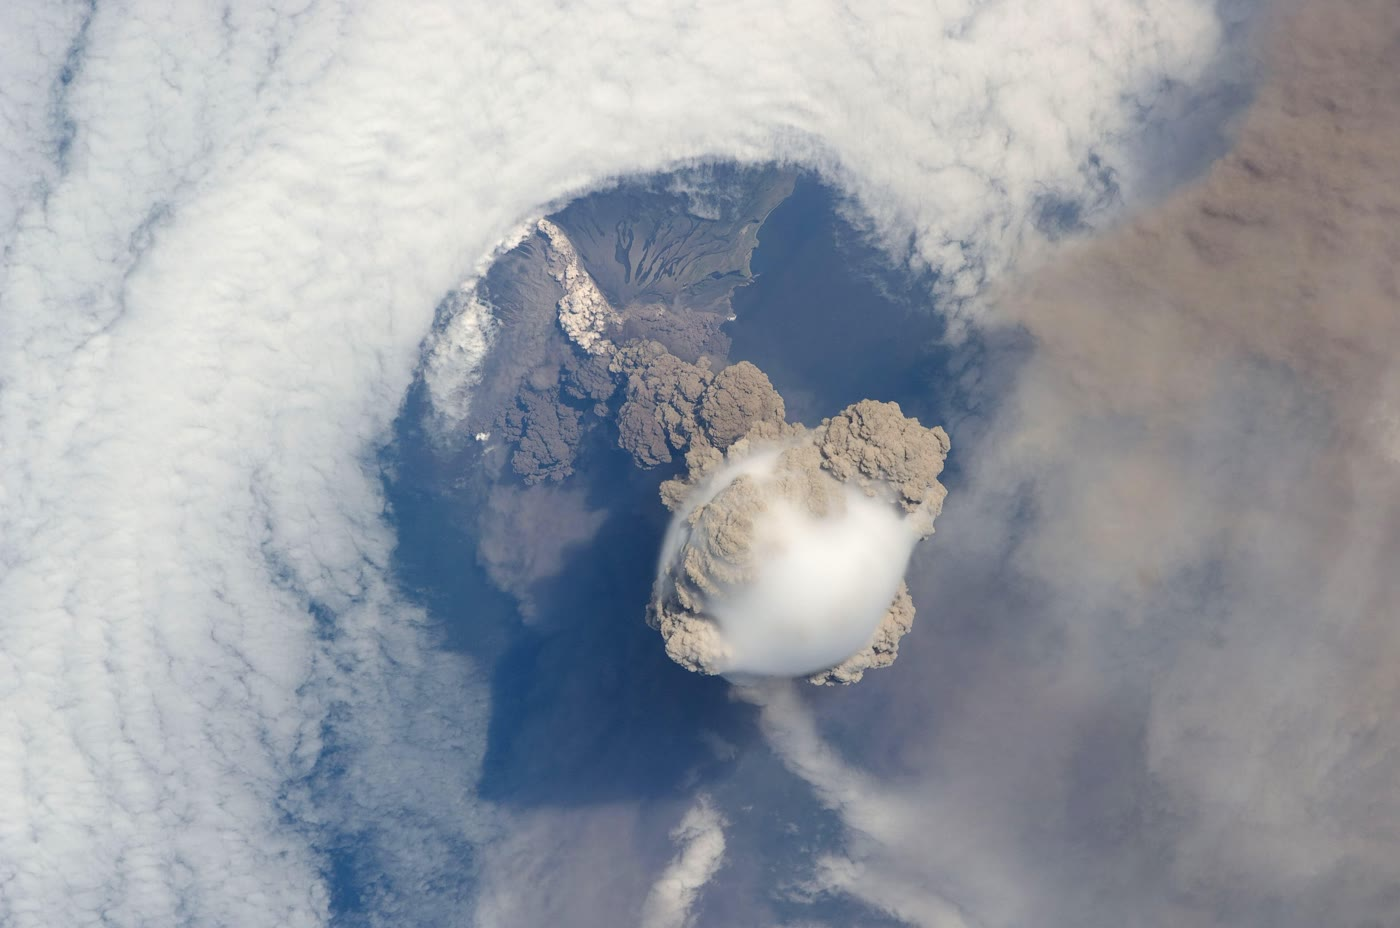
\includegraphics[width=0.66\linewidth]{images/book3/b1-sarychev-iss.jpg}
\par\smallskip{\small Sarychev Peak, a volcano of the Kuril arc on Matua
Island, in an early stage of eruption on 12 June 2009, seen from the
International Space Station through a hole in the clouds. Grey ash, probably a
pyroclastic flow, runs down from the summit, and a smooth cap of cloud, a
pileus, sits on the rising column; ash from the eruption was detected more
than \qty{2400}{km} away. Photograph: NASA, public domain (Wikimedia
Commons).}
\label{fig:b1:active-margins:sarychev}
\end{omfigure}
% ledger: nasa:sarychev, commons:sarychev

The \omterm{def:b1:layered-earth:layers}{crust} beneath arcs is thickened both by shortening and by the magma added
from below; beneath the arcs built on continents, such as the Andes, it is
among the thickest on Earth.

Behind some arcs the overriding plate is pulled apart. Dan Karig explained
these marginal basins of the western Pacific within plate tectonics, in 1971:
when the slab sinks steeply and rolls back, the trench and the arc migrate
towards the sinking plate, and the plate behind them is stretched until it
splits, sometimes leaving an extinct remnant arc on the far side. In the plate
model used above, back-arc spreading runs at about \qty{32}{mm.yr^{-1}} in the
Mariana Trough near \ang{18}\,N, and at more than \qty{110}{mm.yr^{-1}} in the
north of the Lau Basin, behind Tonga. Where the slab is shallow, on the
contrary, it drags the overriding plate, whose \omterm{def:b1:layered-earth:layers}{crust} is shortened and
thickened behind the arc, as behind the Andes.
% ledger: karig:marginal-basins, data:pb2002 (ridge_budget.py: Mariana 32.4, Lau 117.5 mm/yr)

\begin{inthefield}[Warning of a tsunami]
A tsunami warning centre has minutes. In 2011 the first warning for the coast
of north-eastern Japan came about three minutes after the earthquake, from a
magnitude based on the short-period seismic waves; for earthquakes of
magnitude 8 or more such a magnitude is underestimated, and so was the height
of the tsunami. The moment magnitude, which does not saturate, took about
fifteen minutes: the broad-band seismometers of Japan had been driven beyond
their range. Since 2013, when the size of so large an earthquake is uncertain,
the first warning assumes the largest earthquake possible there and describes
the tsunami in words, such as ``huge'', rather than with a number, and the
forecasts draw on offshore measurements of the sea itself, from buoys
positioned by satellite and pressure gauges on the sea floor, which see the
wave before it reaches the coast.
% ledger: jma:warning

\smallskip
\begin{center}
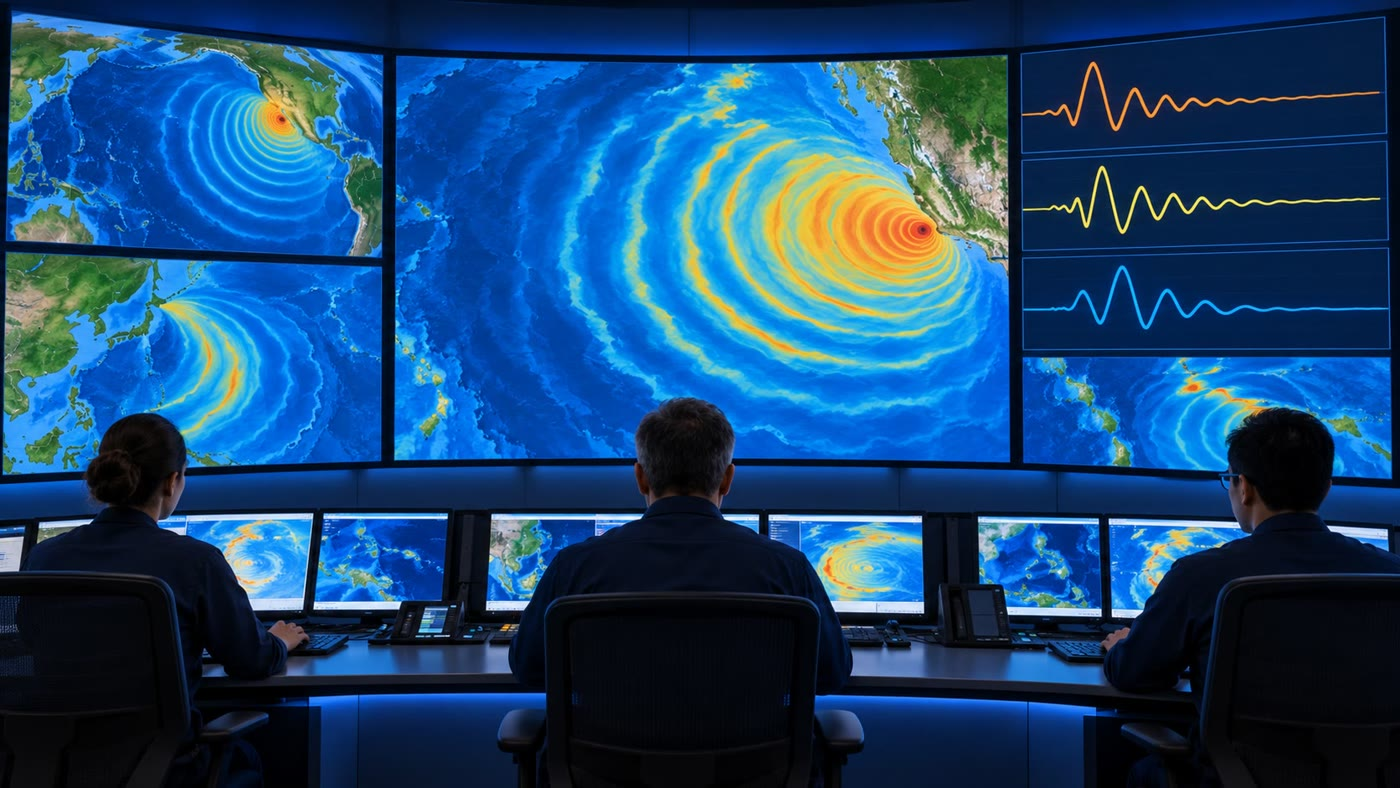
\includegraphics[width=0.7\linewidth]{images/book3/ai/b1-tsunami-centre.jpg}

{\scriptsize Duty officers in a tsunami warning centre, before screens of
computed wave fronts and sea-level records (AI-generated illustration).}
\end{center}
\end{inthefield}

\section{Exercises}

\begin{exercise}[$\star$]\label{exo:b1:active-margins:1}
A trench lies \qty{3}{km} below the ocean floor around it. (a) If it were not
compensated, by how much would the missing rock, of density
\qty{2700}{kg.m^{-3}}, replaced by sea water of density \qty{1000}{kg.m^{-3}},
lower gravity there? Use the Bouguer slab, with
$G = \qty{6.674e-11}{m^3.kg^{-1}.s^{-2}}$. (b) Compare with the observed
anomaly over the Kuril Trench, about \qty{-260}{\milli\gal}, where the trench
lies \qty{3.5}{km} below the floor around it: redo the calculation for that
depth. (c) Why does the water in a trench only tens of kilometres wide give
less than the slab formula, and where must the rest of the deficit lie?
\end{exercise}

\begin{exercise}[$\star$]\label{exo:b1:active-margins:2}
The Pacific plate enters the Kuril Trench at \qty{82}{mm.yr^{-1}}. (a) What
length of plate goes down in 10 million years? (b) If the slab sank along a
straight path dipping \ang{45}, how deep would its leading edge then be? (c)
How long does it take to reach \qty{600}{km}?
\end{exercise}

\begin{exercise}[$\star$]\label{exo:b1:active-margins:3}
Volcanoes stand above the place where a straight slab is \qty{110}{km} deep.
Compute the \omterm{def:b1:active-margins:volcanic-arc}{arc--trench gap} for a slab dipping \ang{30}, \ang{45} and
\ang{60}. Which arc lies farthest from its trench?
\end{exercise}

\begin{exercise}[$\star$]\label{exo:b1:active-margins:4}
In the digital plate model of the chapter, about \qty{2.7}{km^2} of ocean
floor go down the subduction boundaries each year, along about
\qty{51000}{km}, and about \qty{3.0}{km^2} are made along about
\qty{67000}{km} of spreading ridges. (a) Compute the mean convergence rate and
the mean \omterm{def:b1:plate-kinematics:spreading-rate}{full spreading rate}, in \unit{mm.yr^{-1}}. (b) Over all its
boundaries the model destroys as much area as it makes. Where does the rest of
the new floor go?
% ledger: data:pb2002 (ridge_budget.py: 2.739 km2 over 51471 km; 3.009 km2 over 67340 km; all 3.511 vs 3.519)
\end{exercise}

\begin{exercise}[$\star\star$]\label{exo:b1:active-margins:5}
Four earthquakes of a section lie at $(x, z) = (200, 150)$, $(300, 250)$,
$(400, 330)$ and $(500, 430)$, in kilometres. (a) Fit the slab line by least
squares and give its \omterm{def:b1:geological-maps:attitude}{dip}. (b) Where does the line reach the surface? (c)
Compare with the \omterm{def:b1:geological-maps:attitude}{dip} of the line through the first and last earthquakes only.
\end{exercise}

\begin{exercise}[$\star\star$]\label{exo:b1:active-margins:6}
A model slab \omterm{def:b1:geological-maps:attitude}{dips} \ang{25} from the trench down to \qty{50}{km}, then
\ang{45}. The volcanic front stands where the slab is \qty{110}{km} deep. (a)
Compute the \omterm{def:b1:active-margins:volcanic-arc}{arc--trench gap}. (b) Compare with a slab dipping \ang{45} all the
way. (c) The deep segment, extended upwards, reaches the surface: where? Compare
with the Kuril line, which reaches it \qty{53}{km} landward of the trench. (d)
What gap would a deep segment of \ang{60} give?
\end{exercise}

\begin{exercise}[$\star\star$]\label{exo:b1:active-margins:7}
(a) By the bent-shell proposition, what angular radius, and what radius in
kilometres ($R = \qty{6371}{km}$), should an arc have above a slab dipping
\ang{45}? \ang{30}? \ang{70}? (b) Which arcs are the most tightly curved? (c)
The Kuril slab \omterm{def:b1:geological-maps:attitude}{dips} \ang{44.9} and the Kuril Trench fits a circle of
\ang{21.9}: compute the relative difference from the prediction.
\end{exercise}

\begin{exercise}[$\star\star$]\label{exo:b1:active-margins:8}
Take a conductivity of \qty{2.5}{W.m^{-1}.K^{-1}} and a surface temperature
of \qty{10}{\celsius}. (a) Compute the surface temperature gradient beneath a
\omterm{def:b1:active-margins:active-margin}{forearc} losing \qty{35}{mW.m^{-2}} and beneath a back-arc losing
\qty{80}{mW.m^{-2}}. (b) Extrapolating these gradients linearly, estimate the
temperature at \qty{30}{km} in each. (c) Back-arc \omterm{def:b1:layered-earth:discontinuity}{Mohos} are measured at 800 to
\qty{900}{\celsius}. Why is the linear estimate too high?
% ledger: hyndman:backarc (back-arc 70-85, Moho 800-900); the forearc value is an exercise value
\end{exercise}

\begin{exercise}[$\star\star$]\label{exo:b1:active-margins:9}
In the plate model of the chapter, the Mariana Trough opens near \ang{18}\,N at
a full rate of about \qty{32}{mm.yr^{-1}}. (a) Express this rate in
\unit{km.Myr^{-1}}, and give the half-rate if the spreading is symmetric.
(b) How long would the trough take to open by \qty{100}{km} at this rate?
(c) Give two reasons why the age of a \omterm{def:b1:active-margins:active-margin}{back-arc basin} cannot simply be read
from its width and its present rate.
% ledger: data:pb2002 (ridge_budget.py: mariana_18n_mm_yr 32.4)
\end{exercise}

\begin{exercise}[$\star\star\star$]\label{exo:b1:active-margins:10}
A slab \qty{100}{km} thick sinks at \qty{82}{mm.yr^{-1}} along a path dipping
\ang{45}. Take $\kappa = \qty{e-6}{m^2.s^{-1}}$. (a) How long does it take to
reach \qty{600}{km}? (b) How far does heat diffuse into it in that time, by
$\sqrt{\kappa t}$? (c) How long would heat take to reach its middle? (d)
Conclude about the temperature of the slab at \qty{600}{km} and about its
earthquakes.
\end{exercise}

\begin{exercise}[$\star\star\star$]\label{exo:b1:active-margins:11}
A model \omterm{def:b1:active-margins:accretionary}{accretionary prism} has a triangular section: its surface slopes at
$\alpha = \ang{4}$ towards the trench and its base \omterm{def:b1:geological-maps:attitude}{dips} at $\beta = \ang{6}$
beneath it, both meeting at its toe; it keeps these angles as it grows. (a)
Show that its area is $A = \frac12 L^2(\tan\alpha + \tan\beta)$ for a width
$L$, when the angles are small enough for the height at the back to be
$L(\tan\alpha + \tan\beta)$. (b) Sediment \qty{1}{km} thick arrives on a plate
converging at \qty{40}{mm.yr^{-1}}, and all of it is accreted: compute the
width after 1, 4 and 10 million years. How does $L$ grow with time? (c) What
if half the sediment goes down with the slab?
\end{exercise}

\begin{exercise}[$\star\star\star$]\label{exo:b1:active-margins:12}
(a) Show that the least-squares line passes through the mean point
$(\bar x, \bar z)$. (b) A catalogue lists every depth \qty{10}{km} too deep.
How do the slope and the intercept of the fitted line change? (c) The distances
$x$ are all measured from a trench point placed \qty{20}{km} too far
landward, so that every $x$ is \qty{20}{km} too small. How do the slope and
the intercept change? (d) Does either error change the \omterm{def:b1:geological-maps:attitude}{dip}?
\end{exercise}

\section{Problem: Reading a subduction zone from its earthquakes}

\begin{problem}[{Weekend problem --- the Kuril slab from eight earthquakes, how
fast it goes down, what its gravity and heat flow say, and where its volcanoes
should stand}]
\label{pb:b1:active-margins:1}
% values: calc/ch14.py; the eight events are real (USGS catalogue, rounded to the km)
% from figdata/out/bachelor-1-slab_seismicity-section.dat
% ledger: data:b3-usgs-kuril, data:pb2002, data:b2-seafloor-age, syracuse:arc-depth, frank:arcs,
% data:b3-grav-kuril, parsons:plate-model, hyndman:backarc; the forearc heat flow is an exercise value
Eight earthquakes of the Kuril slab, all deeper than \qty{70}{km}, are listed
by their distance $x$ from the trench along the section line, towards the Sea
of Okhotsk, and their depth $z$, both rounded to the kilometre.

\begin{center}
\small
\begin{tabular}{lcccccccc}
\hline
event & 1 & 2 & 3 & 4 & 5 & 6 & 7 & 8\\
$x$ (\unit{km}) & 155 & 222 & 305 & 319 & 431 & 533 & 578 & 609\\
$z$ (\unit{km}) & 96 & 169 & 245 & 272 & 389 & 489 & 518 & 573\\
magnitude & 5.5 & 5.1 & 5.0 & 5.4 & 5.3 & 5.3 & 5.2 & 6.4\\
\hline
\end{tabular}
\end{center}

\medskip
\noindent\textbf{Part I --- The slab line.}
\begin{enumerate}
  \item Plot the eight earthquakes at the same scale on both axes, depth
        downwards.
  \item Compute $\sum x_i$, $\sum z_i$, $\sum x_i^2$, $\sum x_i z_i$ and the
        means $\bar x$ and $\bar z$.
  \item Compute $S_{xx}$ and $S_{xz}$, then the slope of the least-squares line
        to three decimals and its intercept to one decimal.
  \item What is the \omterm{def:b1:geological-maps:attitude}{dip} of the slab?
  \item Where does the line reach the surface? What does this say about the
        shape of the slab near the trench?
  \item Compute the misfit $z_i - (a + s x_i)$ of each earthquake. Which lie
        farthest from the line, and how far?
\end{enumerate}

\medskip
\noindent\textbf{Part II --- How fast the slab goes down.} At the start of the
section the PB2002 model gives a convergence of \qty{87.4}{mm.yr^{-1}}: relative
to the Okhotsk plate, the Pacific plate moves towards \omterm{def:b1:spherical-astronomy:horizontal}{azimuth} \ang{300}. The
section line, perpendicular to the trench, runs towards \omterm{def:b1:spherical-astronomy:horizontal}{azimuth} \ang{320.9}.
\begin{enumerate}[resume]
  \item Compute the angle between the convergence and the section line, then
        the components of the convergence perpendicular and parallel to the
        trench.
  \item What length of plate goes down the trench in 10 million years?
  \item Using the \omterm{def:b1:geological-maps:attitude}{dip} of question 4 (rounded to \ang{45}), how long does the
        slab take to carry a point of its top from the trench down to the
        deepest earthquake of the band, \qty{632}{km}? Neglect the gentler
        \omterm{def:b1:geological-maps:attitude}{dip} near the trench.
  \item The plate is about \qty{122}{Myr} old at the trench. How old is the
        sea floor that is now \qty{632}{km} deep?
  \item By $\sqrt{\kappa t}$, with $\kappa = \qty{e-6}{m^2.s^{-1}}$, how far
        has heat diffused into the slab during that descent? Compare with its
        thickness, about \qty{100}{km}.
\end{enumerate}

\medskip
\noindent\textbf{Part III --- Gravity and heat flow.} Take a conductivity of
\qty{2.5}{W.m^{-1}.K^{-1}}.
\begin{enumerate}[resume]
  \item The old ocean floor in front of the trench loses about
        \qty{43}{mW.m^{-2}}, the back-arc about \qty{80}{mW.m^{-2}}; take
        \qty{35}{mW.m^{-2}} for the \omterm{def:b1:active-margins:active-margin}{forearc}. Compute the temperature gradient
        near the surface of each.
  \item Explain why the \omterm{def:b1:active-margins:active-margin}{forearc} loses less heat than the old ocean floor in
        front of it.
  \item The \omterm{def:b1:isostasy-gravity:anomalies}{free-air anomaly} over the Kuril Trench is about
        \qty{-260}{\milli\gal}. What thickness of rock, \qty{1700}{kg.m^{-3}}
        denser than water, would a Bouguer slab need to give this deficit?
        Compare with the depth of the trench below the floor around it,
        about \qty{3.5}{km}.
  \item Suppose now that the whole plate is pushed down by \qty{3.5}{km}:
        water takes the place of rock at its top, and its \omterm{def:b1:layered-earth:layers}{crust} takes the
        place of \omterm{def:b1:layered-earth:layers}{mantle} at its base, so that, in all, \omterm{def:b1:layered-earth:layers}{mantle} of density
        \qty{3300}{kg.m^{-3}} is replaced by water. Compute the Bouguer slab
        anomaly. Why does the real trench, only tens of kilometres wide, give
        less?
  \item The trench and the outer rise are not in isostatic equilibrium. What
        holds them out of it?
\end{enumerate}

\medskip
\noindent\textbf{Part IV --- Where the volcanoes should stand.} Use the line
of question 3, with its rounded slope and intercept.
\begin{enumerate}[resume]
  \item The first volcano of the band is \qty{164}{km} from the trench. How
        deep is the slab beneath it?
  \item Is this depth within the range found beneath arcs, 72 to
        \qty{173}{km}? How far is it from the average, \qty{105}{km}?
  \item At what distance from the trench is the slab \qty{100}{km} deep?
  \item By the bent-shell proposition, what angular radius should the Kuril
        arc have, and what radius in kilometres?
  \item The Kuril Trench fits a \omterm{def:b1:spherical-astronomy:spherical-triangle}{small circle} of \ang{21.9}. Compare.
  \item Arc volcanoes stand, on average, where the slab is about
        \qty{105}{km} deep. At what distance from the trench does the slab line
        reach that depth?
  \item Compare this distance with the observed \qty{164}{km}: by how many
        kilometres and by what fraction does it differ?
  \item To the nearest kilometre, what \omterm{def:b1:active-margins:volcanic-arc}{arc--trench gap} does the Kuril slab line
        predict for volcanoes standing above the slab at \qty{105}{km}?
\end{enumerate}
\end{problem}
